\documentclass[tikz,convert={density=300,outext=.png}]{standalone}
\usepackage{amsmath}
\usetikzlibrary{arrows.meta,graphs}
\definecolor{wbl.fg}{rgb}{1.0, 0.5, 0.31}
\definecolor{wbl.bg}{rgb}{0.15, 0.38, 0.61}
\begin{document}
  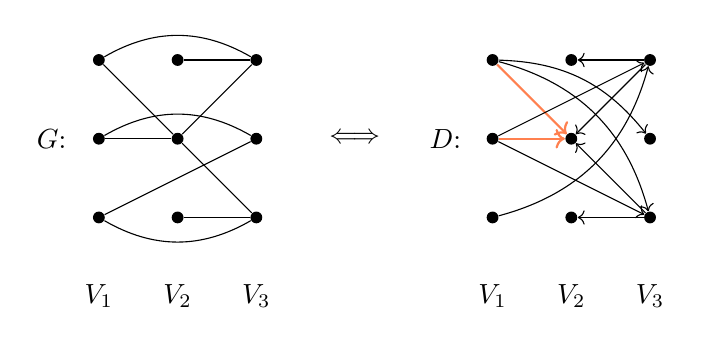
\begin{tikzpicture}
  \tikzset{circ/.append style={circle, fill=black, inner sep = 0,
      minimum size = 0.15cm}}
  \node[circ] (1) at (0,0) {};
  \node[circ] (2) at (0,1) {};
  \node[circ] (3) at (0,2) {};
  \node[circ] (4) at (1,0) {};
  \node[circ] (5) at (1,1) {};
  \node[circ] (6) at (1,2) {};
  \node[circ] (7) at (2,0) {};
  \node[circ] (8) at (2,1) {};
  \node[circ] (9) at (2,2) {};

  \node (g) at (-.6, 1) {$G$:};
  \node (v1) at (0,-1) {$V_1$};
  \node (v2) at (1,-1) {$V_2$};
  \node (v3) at (2,-1) {$V_3$};
  
  \graph[use existing nodes] {
    3 --[bend left] 9;
    2 -- 5 -- 9;
    3 -- 5 -- 7 --[bend left] 1 -- 8 --[bend right] 2;
    4 -- 7;
    6 -- 9;
  };

  \node (arr) at (3.25,1) {$\Longleftrightarrow$};

  \node[circ] (1) at (0+5,0) {};
  \node[circ] (2) at (0+5,1) {};
  \node[circ] (3) at (0+5,2) {};
  \node[circ] (4) at (1+5,0) {};
  \node[circ] (5) at (1+5,1) {};
  \node[circ] (6) at (1+5,2) {};
  \node[circ] (7) at (2+5,0) {};
  \node[circ] (8) at (2+5,1) {};
  \node[circ] (9) at (2+5,2) {};

  \node (gp) at (-.6+5,1) {$D$:};
  \node (v1) at (0+5,-1) {$V_1$};
  \node (v2) at (1+5,-1) {$V_2$};
  \node (v3) at (2+5,-1) {$V_3$};
  
  \graph[use existing nodes] {
    3 ->[thick, wbl.fg] 5;
    2 ->[thick, wbl.fg] 5;
    2 -> 9;
    1 ->[bend right] 9;
    9 -> 5;
    7 -> 5;
    2 -> 7;
    3 ->[bend left] 7;
    7 -> 4;
    3 -> [bend left=25] 8;
    9 -> 6;
  };
  \end{tikzpicture}
\end{document}



